\documentclass[12pt]{article} % use larger type; default would be 10pt

\usepackage{tikz}
\usepackage{pgfplots}
\usetikzlibrary{calc}
\usetikzlibrary{arrows.meta}
\usetikzlibrary{patterns}
        \newcommand\degree[0]{^{\circ}}
\usetikzlibrary{shapes.misc}

\title{Play with TikZ}
\author{Just Us}
%\date{} % Activate to display a given date or no date (if empty),
         % otherwise the current date is printed 

\begin{document}
\maketitle

\section{Chap 5 Equations and Identities}

\subsection{5.3 Trigonometric Identities}

fig-5-3-abs $y=\sqrt{x^2}$ and $y=x$
\begin{tikzpicture} [scale=.5]
\coordinate (O) at (0,0);
\coordinate (B) at ($ (O)+(0,-4) $);
\draw[black, thick] (O)++(-4.7,0)--++(9.4,0);
\draw[black, thick] (O)++(0,-3.1)--++(0,6.2);
\draw[blue, thick] (O)++(-3.1,3.1)--(O)--++(3.1,3.1);
\node[text width = 1.8cm] at (B) {\color{blue}$Y_1=\sqrt{x^2}$};

\coordinate (O) at (11,0);
\coordinate (B) at ($ (O)+(0,-4) $);
\draw[black, thick] (O)++(-4.7,0)--++(9.4,0);
\draw[black, thick] (O)++(0,-3.1)--++(0,6.2);
\draw[blue, thick] (O)++(-3.1,-3.1)--(O)--++(3.1,3.1);
\node[text width = 1.4cm] at (B) {\color{blue}$Y_2=x$};
\end{tikzpicture}
\newline

fig-5-3-abs v2 $y=\sqrt{x^2}$ and $y=x$
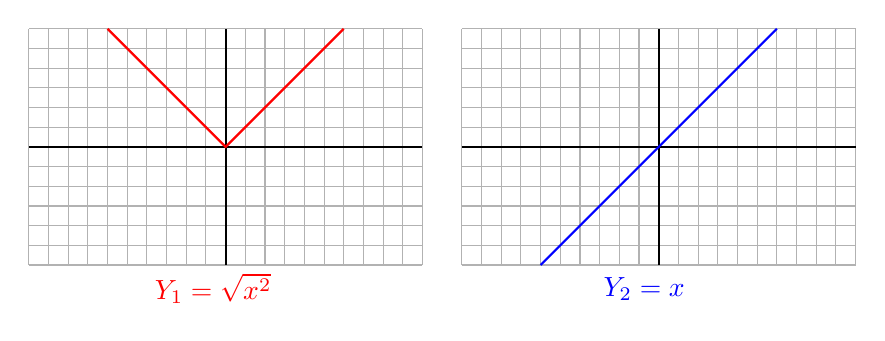
\begin{tikzpicture} [scale=.25]

\draw[gray!60] (-10,-6) grid (10,6);
\coordinate (O) at (0,0);
\coordinate (B) at ($ (O)+(0,-7.2) $);
\draw[black, thick] (O)++(-10,0)--++(20,0);
\draw[black, thick] (O)++(0,-6)--++(0,12);
\draw[red, thick] (O)++(-6,6)--(O)--++(6,6);
\node[text width = 1.8cm] at (B) {\color{red}$Y_1=\sqrt{x^2}$};

\draw[gray!60] (12,-6) grid (32,6);
\coordinate (O) at (22,0);
\coordinate (B) at ($ (O)+(0,-7.2) $);
\draw[black, thick] (O)++(-10,0)--++(20,0);
\draw[black, thick] (O)++(0,-6)--++(0,12);
\draw[blue, thick] (O)++(-6,-6)--(O)--++(6,6);
\node[text width = 1.4cm] at (B) {\color{blue}$Y_2=x$};
\end{tikzpicture}
\newline

exam5-3-3a don't use
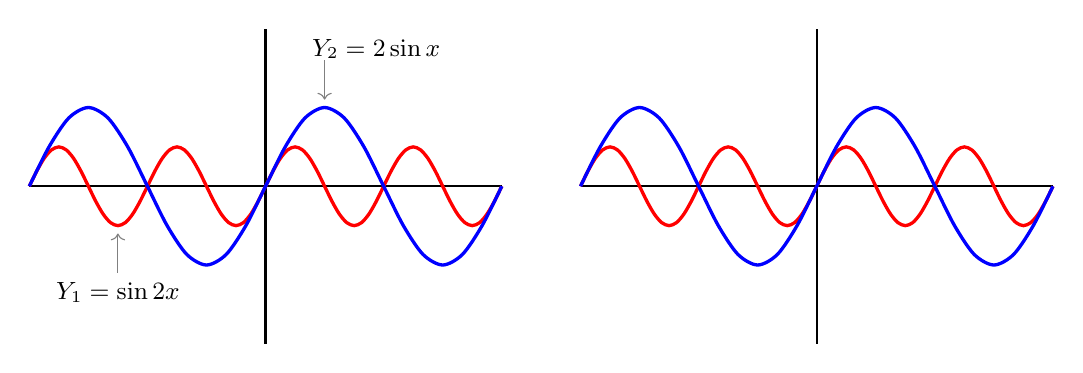
\begin{tikzpicture} [xscale=.25, yscale=.5]

\coordinate (O) at (0,0);
\coordinate (B) at ($ (O)+(0,-7.2) $);
\draw[black, thick] (O)++(-12,0)--++(24,0);
\draw[black, thick] (O)++(0,-4)--(0,4);
\draw[samples=65,domain=-12:12,smooth,variable=\x,red,very thick] plot ({\x},{sin( 2*30*\x )});
\draw[domain=-12:12,smooth,variable=\x,blue,very thick] plot ({\x},{ 2*sin( 30*\x )});
\draw[gray, <-] (-7.5,-1.2)--++(0,-1.) node[below] {\small\color{black}$Y_1= \sin 2x$};
\draw[gray, <-] (3,2.2)--++(0,1.) node[above right, xshift=-8, yshift=-3] {\small\color{black}$Y_2= 2 \sin x$};

\coordinate (O) at (28,0);
\coordinate (B) at ($ (O)+(0,-7.2) $);
\draw[black, thick] (O)++(-12,0)--++(24,0);
\draw[black, thick] (O)++(0,-4)--++(0,8);
\draw[samples=65,domain=16:40,smooth,variable=\x,red,very thick] plot ({\x},{sin( 2*30*(\x-28) )});
\draw[domain=16:40,smooth,variable=\x,blue,very thick] plot ({\x},{ 2*sin( 30*(\x-28) )});
\end{tikzpicture}
\newline

exam5-3-7
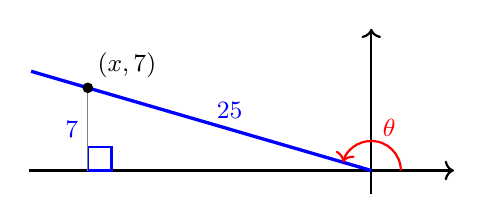
\begin{tikzpicture} [scale=.15]

\coordinate (O) at (0,0);
\coordinate (A) at (-24,7);
\coordinate (B) at (-24,0);
\draw[black, thick, ->] (-29,0) -- (7,0);
\draw[black, thick, ->] (0,-2) -- (0,12);
\draw[blue, very thick] (O)--(A) node [above, midway] {\small 25};
\draw[blue, very thick] (A)--+(-4.8, 1.4);

\draw[blue, thick] (B) rectangle ++(2,2);
\draw[gray] (A)--(B) node[left, midway] {\small \color{blue} 7};
\filldraw[black] (A) circle (.4cm) node[anchor=south west]{\small $(x,7)$};
\draw[red, thick, ->] (2.5,0) arc (0:{180-atan(7/24)}:2.5) node[above, midway, xshift=5, yshift=-2] {\small $\theta$};

\end{tikzpicture}
\newline

exam5-3-9
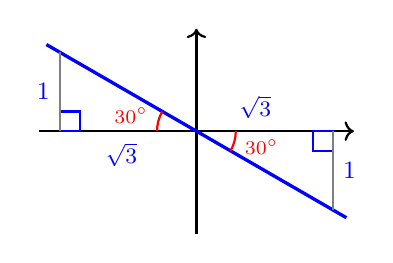
\begin{tikzpicture} 
\coordinate (O) at (0,0);
\coordinate (A) at ($ sqrt(3)*(1,0)  $);
\coordinate (B) at ($ sqrt(3)*(-1,0)  $);
\coordinate (Ap) at (-30:2.2);
\coordinate (Bp) at (150:2.2);

\draw[black, thick, ->] (-2,0) -- (2,0);
\draw[black, thick, ->] (0,-1.3) -- (0,1.3);
\draw[blue, very thick] (Ap)--(Bp);

\draw[blue, thick] (A) rectangle ++(-.25,-.25);
\draw[blue, thick] (B) rectangle ++(.25,.25);
\draw[gray, thick] (A)--++(0,-1) node[right, midway] {\small \color{blue} 1};
\draw[gray,thick] (B)--++(0,1) node[left, midway] {\small \color{blue} 1};

\draw[red, thick] (-.5,0) arc (180:150:.5) node[left, midway, yshift=2 ] {\scriptsize $30\degree$};
\draw[red, thick] (.5,0) arc (0:-30:.5) node[right, midway, yshift=-2 ] {\scriptsize $30\degree$};

\node[text width=.7cm] at (.9,.3) {\color{blue}\footnotesize$\sqrt{3}$};
\node[text width=.7cm] at (-.8,-.3) {\color{blue}\footnotesize$\sqrt{3}$};

\end{tikzpicture}
\newline

ch6-4

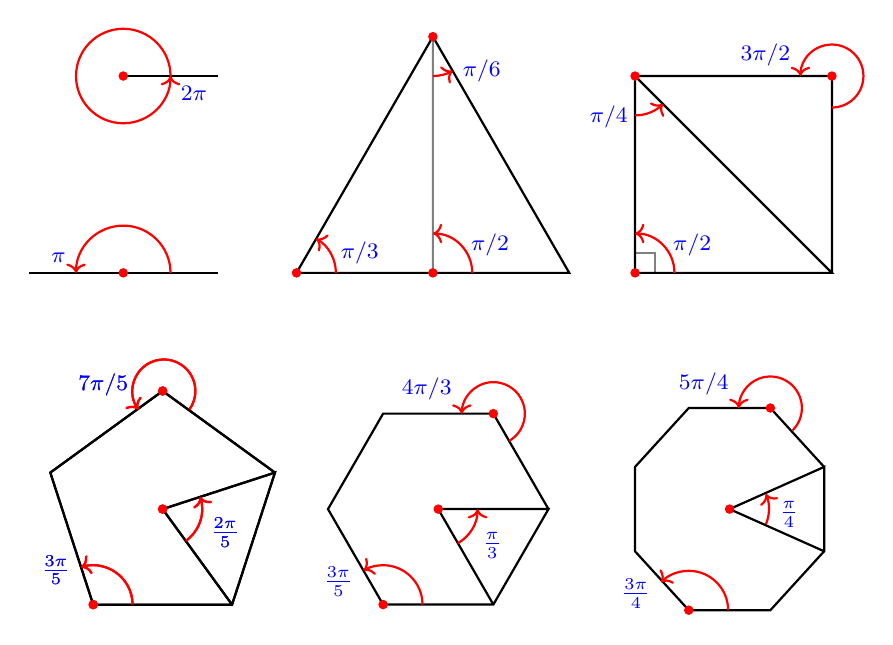
\begin{tikzpicture} 
\coordinate (O) at (0,0);
\coordinate (A) at (0,2.5);
\draw[black, thick] (A)--++(1.2,0);
\filldraw[red] (A) circle (1.5pt);
\draw[red, thick, ->] (.6,2.5) arc (0:360:.6cm) node[below right]{\color{blue}\footnotesize $2\pi$};

%second fig
\draw[black, thick] (-1.2,0)--(1.2,0);
\filldraw[red] (O) circle (1.5pt);
\draw[red, thick, ->] (.6,0) arc (0:180:.6cm) node[above left]{\color{blue}\footnotesize $\pi$};

%third fig
\coordinate (O) at (2.2,0);
\coordinate (A) at ($ (O) + 2*sqrt(3)*(1,0) $);
\coordinate (B) at ($ (A)+ sqrt(3)*(-1,0)+(0,3) $);
\coordinate (C) at ($ (O)+ sqrt(3)*(1,0) $);
\draw[black, thick] (O)--(A) -- (B)--(O);
\draw[gray, thick] (B)--(C);
\filldraw[red] (O) circle (1.5pt);
\draw[red, thick, ->] (2.7,0) arc (0:60:.5cm) node[right, midway]{\color{blue}\footnotesize $\pi/3$};
\filldraw[red] (C) circle (1.5pt);
\draw[red, thick, ->] ($ (C) + (.5,0) $) arc (0:90:.5cm) node[right, midway]{\color{blue}\footnotesize $\pi/2$};
\filldraw[red] (B) circle (1.5pt);
\draw[red, thick, ->] ($ (B) + (0, -.5) $) arc (-90:-60:.5cm) node[ right, ]{\color{blue}\footnotesize $\pi/6$};

%fourth fig
\coordinate (O) at (6.5,0);
\coordinate (A) at ($ (O) +(2.5,0) $);
\coordinate (B) at ($ (A)+ (0,2.5) $);
\coordinate (C) at ($ (O) + (0,2.5) $);
\draw[gray, thick] (O) rectangle ++(.25,.25);
\draw[black, thick] (A) -- (B)-- (C)--(O)--(A)--(C);

\filldraw[red] (O) circle (1.5pt);
\draw[red, thick, ->] ($ (O) + (.5,0)$) arc (0:90:.5cm) node[right, midway]{\color{blue}\footnotesize $\pi/2$};
\filldraw[red] (C) circle (1.5pt);
\draw[red, thick, ->] ($ (C) + (0,-.5)$) arc (-90:-45:.5cm) node[anchor=north east, xshift=-9, yshift=3]{\color{blue}\footnotesize $\pi/4$};
\filldraw[red] (B) circle (1.5pt);
\draw[red, thick, ->] ($ (B) + (0,-.4)$) arc (-90:180:.4cm) node[anchor=south east, ]{\color{blue}\footnotesize $3\pi/2$};

%fifth fig
\coordinate (O) at (.5,-3);
\coordinate (A) at ($ (O) +1.5*(0,1) $);
\coordinate (B) at ($ (O)+1.5*cos(72)*(0,1) +1.5*sin(72)*(-1,0) $);
\coordinate (C) at ($ (O)+1.5*cos(36)*(0,-1) +1.5*sin(36)*(-1,0) $);
\coordinate (D) at ($ (O)+1.5*cos(36)*(0,-1) +1.5*sin(36)*(1,0) $);
\coordinate (E) at ($ (O)+1.5*cos(72)*(0,1) +1.5*sin(72)*(1,0) $);

\draw[black, thick] (E)--(A)-- (B)-- (C)--(D)--(E)--(O)--(D);

\filldraw[red] (O) circle (1.5pt);
\draw[red, thick, ->] ($ (O) + .5*sin(36)*(1,0) + .5*cos(36)*(0,-1)$) arc (-54:18:.5cm) node[right, midway, yshift=-4]{\color{blue}\small $\frac{2\pi}{5}$};
\filldraw[red] (C) circle (1.5pt);
\draw[red, thick, ->] ($ (C) + (.5,0)$) arc (0:108:.5cm) node[anchor=north east, yshift=8]{\color{blue}\small $\frac{3\pi}{5}$};
\filldraw[red] (A) circle (1.5pt);
\draw[red, thick, ->] ($ (A) + 0.4*sin(36)*(0,-1) + .4*cos(32)*(1,0)$) arc (-36:216:.4cm) node[anchor=south east, yshift=1]{\color{blue}\footnotesize $7\pi/5$};

%sixth fig
\coordinate (O) at (4,-3);
\coordinate (A) at ($ (O) +1.4*(1,0) $);
\coordinate (B) at ($ (O)+1.4*cos(60)*(1,0) +1.4*sin(60)*(0,1) $);
\coordinate (C) at ($ (O)+1.4*cos(60)*(-1,0) +1.4*sin(60)*(0,1) $);
\coordinate (D) at ($ (O)+1.4*(-1,0) $);
\coordinate (E) at ($ (O)+1.4*cos(60)*(-1,0) +1.4*sin(60)*(0,-1) $);
\coordinate (F) at ($ (O)+1.4*cos(60)*(1,0) +1.4*sin(60)*(0,-1) $);

\draw[black, thick] (A)-- (B)-- (C)--(D)--(E)--(F)--(A)--(O)--(F);

\filldraw[red] (O) circle (1.5pt);
\draw[red, thick, <-] ($ (O) + .5*(1,0) $) arc (0:-60:.5cm) node[right, midway, yshift=-6]{\color{blue}\small $\frac{\pi}{3}$};
\filldraw[red] (E) circle (1.5pt);
\draw[red, thick, ->] ($ (E) + (.5,0)$) arc (0:120:.5cm) node[left, yshift=-4]{\color{blue}\small $\frac{3\pi}{5}$};
\filldraw[red] (B) circle (1.5pt);
\draw[red, thick, ->] ($ (B) + 0.4*sin(60)*(0,-1) + .4*cos(60)*(1,0)$) arc (-60:180:.4cm) node[anchor=south east, yshift=1]{\color{blue}\footnotesize $4\pi/3$};


%fifth fig
\coordinate (O) at (.5,-3);
\coordinate (A) at ($ (O) +1.5*(0,1) $);
\coordinate (B) at ($ (O)+1.5*cos(72)*(0,1) +1.5*sin(72)*(-1,0) $);
\coordinate (C) at ($ (O)+1.5*cos(36)*(0,-1) +1.5*sin(36)*(-1,0) $);
\coordinate (D) at ($ (O)+1.5*cos(36)*(0,-1) +1.5*sin(36)*(1,0) $);
\coordinate (E) at ($ (O)+1.5*cos(72)*(0,1) +1.5*sin(72)*(1,0) $);

\draw[black, thick] (E)--(A)-- (B)-- (C)--(D)--(E)--(O)--(D);

\filldraw[red] (O) circle (1.5pt);
\draw[red, thick, ->] ($ (O) + .5*sin(36)*(1,0) + .5*cos(36)*(0,-1)$) arc (-54:18:.5cm) node[right, midway, yshift=-4]{\color{blue}\small $\frac{2\pi}{5}$};
\filldraw[red] (C) circle (1.5pt);
\draw[red, thick, ->] ($ (C) + (.5,0)$) arc (0:108:.5cm) node[anchor=north east, yshift=8]{\color{blue}\small $\frac{3\pi}{5}$};
\filldraw[red] (A) circle (1.5pt);
\draw[red, thick, ->] ($ (A) + 0.4*sin(36)*(0,-1) + .4*cos(32)*(1,0)$) arc (-36:216:.4cm) node[anchor=south east, yshift=1]{\color{blue}\footnotesize $7\pi/5$};

%seventh fig
\coordinate (O) at (7.7,-3);
\coordinate (A) at ($ (O) +1.3*cos(22.5)*(1,0) +1.4*sin(22.5)*(0,1) $);
\coordinate (B) at ($ (O)+1.3*cos(66.5)*(1,0) +1.4*sin(66.5)*(0,1) $);
\coordinate (C) at ($ (O)+1.3*cos(66.5)*(-1,0) +1.4*sin(66.5)*(0,1) $);
\coordinate (D) at ($ (O) +1.3*cos(22.5)*(-1,0) +1.4*sin(22.5)*(0,1) $);
\coordinate (E) at ($ (O) +1.3*cos(22.5)*(-1,0) +1.4*sin(22.5)*(0,-1) $);
\coordinate (F) at ($ (O)+1.3*cos(66.5)*(-1,0) +1.4*sin(66.5)*(0,-1)  $);
\coordinate (G) at ($ (O)+1.3*cos(66.5)*(1,0) +1.4*sin(66.5)*(0,-1) $);
\coordinate (H) at ($ (O) +1.3*cos(22.5)*(1,0) +1.4*sin(22.5)*(0,-1) $);

\draw[black, thick] (A)-- (B)-- (C)--(D)--(E)--(F)--(G)--(H)--(A)--(O)--(H);

\filldraw[red] (O) circle (1.5pt);
\draw[red, thick, ->] ($ (O) + .5*cos(22.5)*(1,0)+ .5*sin(22.5)*(0,-1) $) arc (-22.5:22.5:.5cm) node[right, midway, yshift=-2]{\color{blue}\small $\frac{\pi}{4}$};
\filldraw[red] (F) circle (1.5pt);
\draw[red, thick, ->] ($ (F) + (.5,0)$) arc (0:135:.5cm) node[left, yshift=-4]{\color{blue}\small $\frac{3\pi}{4}$};
\filldraw[red] (B) circle (1.5pt);
\draw[red, thick, ->] ($ (B) + 0.4*sin(45)*(0,-1) + .4*cos(45)*(1,0)$) arc (-45:180:.4cm) node[anchor=south east, yshift=1]{\color{blue}\footnotesize $5\pi/4$};

\end{tikzpicture}
\newline

ch6-5

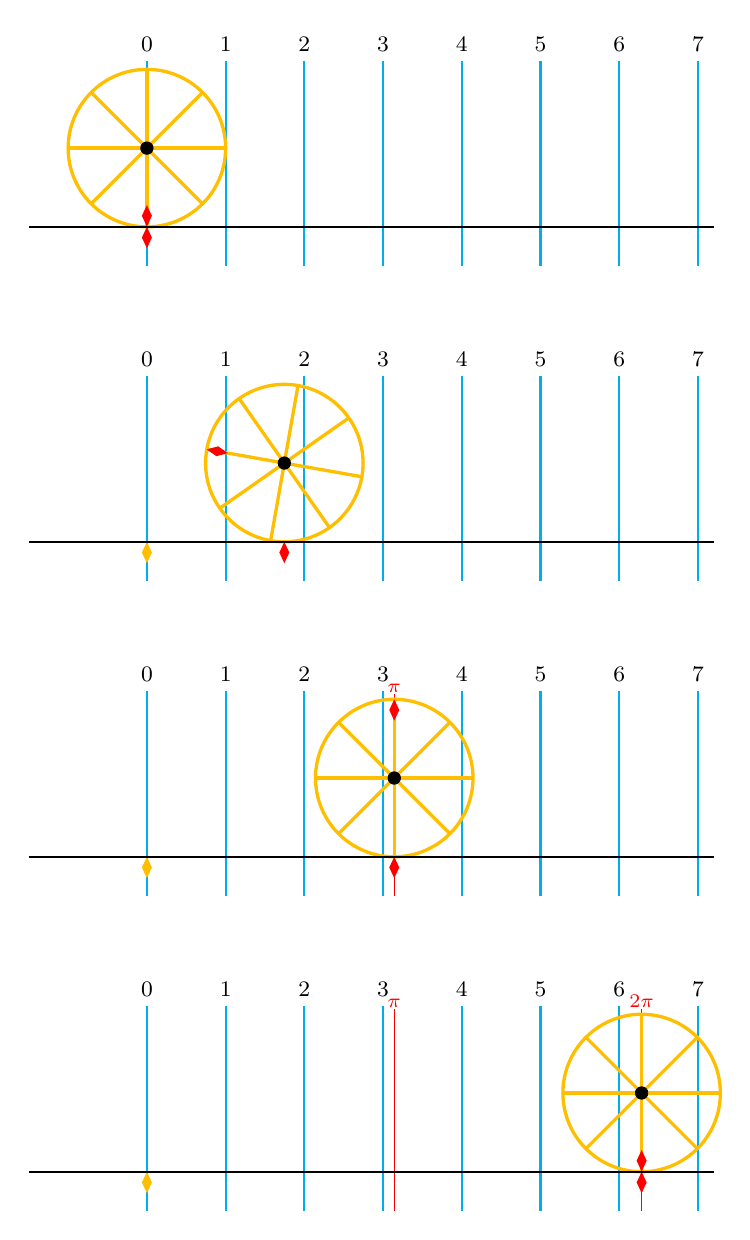
\begin{tikzpicture} 
\coordinate (O) at (0,0);
\coordinate (A) at (0,1);
\coordinate (B) at ($ (A) + cos(0)*(1,0) + sin(0)*(0,1) $);
\coordinate (C) at ($ (A) + cos(45)*(1,0) + sin(45)*(0,1) $);
\coordinate (D) at ($ (A) + cos(90)*(1,0) + sin(90)*(0,1) $);
\coordinate (E) at ($ (A) + cos(135)*(1,0) + sin(135)*(0,1) $);
\coordinate (F) at ($ (A) + cos(180)*(1,0) + sin(180)*(0,1) $);
\coordinate (G) at ($ (A) + cos(225)*(1,0) + sin(225)*(0,1) $);
\coordinate (H) at ($ (A) + cos(270)*(1,0) + sin(270)*(0,1) $);
\coordinate (I) at ($ (A) + cos(315)*(1,0) + sin(315)*(0,1) $);
\foreach \x in {0, 1, ..., 7}
 \draw[cyan, thick] ($ (O)+(\x,-.5) $)--++(0,2.6) node[anchor=south]{\footnotesize\color{black} \x};

\draw[orange!50!yellow, very thick] (A) circle (1cm);
\draw[orange!50!yellow, very thick] (B) -- (F);
\draw[orange!50!yellow, very thick] (C) -- (G);
\draw[orange!50!yellow, very thick] (D) -- (H);
\draw[orange!50!yellow, very thick] (E) -- (I);
\filldraw[black] (A) circle (2.2pt);
\coordinate (P) at ($ (H) + .15*cos(65)*(1,0)+.15*sin(70)*(0,1) $);
\coordinate (Q) at at ($ (P) + .15*cos(65)*(-1,0)+ .15* sin(65)*(0,1) $);
\coordinate (R) at at ($ (Q) + .15* cos(65)*(-1,0)+.15* sin(65)*(0,-1) $);
\draw[draw=none, fill=red] (H)--(P)--(Q)--(R)--cycle;

\coordinate (P) at ($ (H) + .15*cos(65)*(1,0)+.15*sin(65)*(0,-1) $);
\coordinate (Q) at at ($ (P) + .15*cos(65)*(-1,0)+ .15* sin(65)*(0,-1) $);
\coordinate (R) at at ($ (Q) + .15* cos(65)*(-1,0)+ .15* sin(65)*(0,1) $);
\draw[draw=none, fill=red] (H)--(P)--(Q)--(R)--cycle;
\draw[black, thick] (O)+(-1.5,0)--+(7.2,0);

%second fig
\coordinate (O) at (0,-4);
\coordinate (A) at ($ 100*pi/180*(1,0)+(0,-3) $);
\coordinate (B) at ($ (A) + cos(-100)*(1,0) + sin(-100)*(0,1) $);
\coordinate (C) at ($ (A) + cos(-55)*(1,0) + sin(-55)*(0,1) $);
\coordinate (D) at ($ (A) + cos(-10)*(1,0) + sin(-10)*(0,1) $);
\coordinate (E) at ($ (A) + cos(35)*(1,0) + sin(35)*(0,1) $);
\coordinate (F) at ($ (A) + cos(80)*(1,0) + sin(80)*(0,1) $);
\coordinate (G) at ($ (A) + cos(125)*(1,0) + sin(125)*(0,1) $);
\coordinate (H) at ($ (A) + cos(170)*(1,0) + sin(170)*(0,1) $);
\coordinate (I) at ($ (A) + cos(215)*(1,0) + sin(215)*(0,1) $);
\foreach \x in {0, 1, ..., 7}
 \draw[cyan, thick] ($ (O)+(\x,-.5) $)--++(0,2.6) node[anchor=south]{\footnotesize\color{black} \x};

\draw[orange!50!yellow, very thick] (A) circle (1cm);
\draw[orange!50!yellow, very thick] (B) -- (F);
\draw[orange!50!yellow, very thick] (C) -- (G);
\draw[orange!50!yellow, very thick] (D) -- (H);
\draw[orange!50!yellow, very thick] (E) -- (I);
\filldraw[black] (A) circle (2.2pt);
\coordinate (T) at ($ (A) + (0,-1) $);
\coordinate (P) at ($ (H) + .15*cos(-35)*(1,0)+.15* sin(-35)*(0,1) $);
\coordinate (Q) at at ($ (P) + .15*cos(15)*(1,0)+ .15* sin(15)*(0,1) $);
\coordinate (R) at at ($ (Q) + .15* cos(-35)*(-1,0)+.15* sin(-35)*(0,-1) $);
\draw[draw=none, fill=red] (H)--(P)--(Q)--(R)--cycle;
%red diamond on axis
\coordinate (P) at ($ (T) + .15*cos(65)*(1,0)+.15*sin(65)*(0,-1) $);
\coordinate (Q) at at ($ (P) + .15*cos(65)*(-1,0)+ .15* sin(65)*(0,-1) $);
\coordinate (R) at at ($ (Q) + .15* cos(65)*(-1,0)+ .15* sin(65)*(0,1) $);
\draw[draw=none, fill=red] (T)--(P)--(Q)--(R)--cycle;
%yellow diamond on axis
\coordinate (P) at ($ (O) + .15*cos(65)*(1,0)+.15*sin(65)*(0,-1) $);
\coordinate (Q) at at ($ (P) + .15*cos(65)*(-1,0)+ .15* sin(65)*(0,-1) $);
\coordinate (R) at at ($ (Q) + .15* cos(65)*(-1,0)+ .15* sin(65)*(0,1) $);
\draw[draw=none, fill=orange!50!yellow] (O)--(P)--(Q)--(R)--cycle;

\draw[black, thick] (O)+(-1.5,0)--+(7.2,0);

%fourth fig
\coordinate (O) at (0,-12);
\coordinate (A) at ($ 2* pi*(1,0)+(0,-11) $);
\coordinate (B) at ($ (A) + cos(0)*(1,0) + sin(0)*(0,1) $);
\coordinate (C) at ($ (A) + cos(45)*(1,0) + sin(45)*(0,1) $);
\coordinate (D) at ($ (A) + cos(90)*(1,0) + sin(90)*(0,1) $);
\coordinate (E) at ($ (A) + cos(135)*(1,0) + sin(135)*(0,1) $);
\coordinate (F) at ($ (A) + cos(180)*(1,0) + sin(180)*(0,1) $);
\coordinate (G) at ($ (A) + cos(225)*(1,0) + sin(225)*(0,1) $);
\coordinate (H) at ($ (A) + cos(270)*(1,0) + sin(270)*(0,1) $);
\coordinate (I) at ($ (A) + cos(315)*(1,0) + sin(315)*(0,1) $);
\foreach \x in {0, 1, ..., 7}
 \draw[cyan, thick] ($ (O)+(\x,-.5) $)--++(0,2.6) node[anchor=south]{\footnotesize\color{black} \x};

\draw[red] ($ (O)+(2*pi,-.5) $)--++(0,2.57) node[anchor=south, yshift=-3]{\scriptsize $2\pi$};
\draw[red] ($ (O)+(pi,-.5) $)--++(0,2.57) node[anchor=south, yshift=-3]{\scriptsize $\pi$};

\draw[orange!50!yellow, very thick] (A) circle (1cm);
\draw[orange!50!yellow, very thick] (B) -- (F);
\draw[orange!50!yellow, very thick] (C) -- (G);
\draw[orange!50!yellow, very thick] (D) -- (H);
\draw[orange!50!yellow, very thick] (E) -- (I);
\filldraw[black] (A) circle (2.2pt);
\coordinate (T) at ($ (A) + (0,-1) $);
\coordinate (P) at ($ (H) + .15*cos(65)*(1,0)+.15*sin(70)*(0,1) $);
\coordinate (Q) at at ($ (P) + .15*cos(65)*(-1,0)+ .15* sin(65)*(0,1) $);
\coordinate (R) at at ($ (Q) + .15* cos(65)*(-1,0)+.15* sin(65)*(0,-1) $);
\draw[draw=none, fill=red] (H)--(P)--(Q)--(R)--cycle;

%red diamond on axis
\coordinate (P) at ($ (T) + .15*cos(65)*(1,0)+.15*sin(65)*(0,-1) $);
\coordinate (Q) at at ($ (P) + .15*cos(65)*(-1,0)+ .15* sin(65)*(0,-1) $);
\coordinate (R) at at ($ (Q) + .15* cos(65)*(-1,0)+ .15* sin(65)*(0,1) $);
\draw[draw=none, fill=red] (T)--(P)--(Q)--(R)--cycle;
%yellow diamond on axis
\coordinate (P) at ($ (O) + .15*cos(65)*(1,0)+.15*sin(65)*(0,-1) $);
\coordinate (Q) at at ($ (P) + .15*cos(65)*(-1,0)+ .15* sin(65)*(0,-1) $);
\coordinate (R) at at ($ (Q) + .15* cos(65)*(-1,0)+ .15* sin(65)*(0,1) $);
\draw[draw=none, fill=orange!50!yellow] (O)--(P)--(Q)--(R)--cycle;

\draw[black, thick] (O)+(-1.5,0)--+(7.2,0);

%third fig
\coordinate (O) at (0,-8);
\coordinate (A) at ($ pi*(1,0)+(0,-7) $);
\coordinate (B) at ($ (A) + cos(-180)*(1,0) + sin(-180)*(0,1) $);
\coordinate (C) at ($ (A) + cos(-135)*(1,0) + sin(-135)*(0,1) $);
\coordinate (D) at ($ (A) + cos(-90)*(1,0) + sin(-90)*(0,1) $);
\coordinate (E) at ($ (A) + cos(-45)*(1,0) + sin(-45)*(0,1) $);
\coordinate (F) at ($ (A) + cos(0)*(1,0) + sin(0)*(0,1) $);
\coordinate (G) at ($ (A) + cos(45)*(1,0) + sin(45)*(0,1) $);
\coordinate (H) at ($ (A) + cos(90)*(1,0) + sin(90)*(0,1) $);
\coordinate (I) at ($ (A) + cos(135)*(1,0) + sin(135)*(0,1) $);
\foreach \x in {0, 1, ..., 7}
 \draw[cyan, thick] ($ (O)+(\x,-.5) $)--++(0,2.6) node[anchor=south]{\footnotesize\color{black} \x};

\draw[red] ($ (O)+(pi,-.5) $)--++(0,2.57) node[anchor=south, yshift=-3]{\scriptsize $\pi$};

\draw[orange!50!yellow, very thick] (A) circle (1cm);
\draw[orange!50!yellow, very thick] (B) -- (F);
\draw[orange!50!yellow, very thick] (C) -- (G);
\draw[orange!50!yellow, very thick] (D) -- (H);
\draw[orange!50!yellow, very thick] (E) -- (I);
\filldraw[black] (A) circle (2.2pt);
\coordinate (T) at ($ (A) + (0,-1) $);
\coordinate (P) at ($ (H) + .15*cos(65)*(1,0)+.15* sin(65)*(0,-1) $);
\coordinate (Q) at at ($ (P) + .15*cos(65)*(-1,0)+ .15* sin(65)*(0,-1) $);
\coordinate (R) at at ($ (Q) + .15* cos(65)*(-1,0)+ .15* sin(65)*(0,1) $);
\draw[draw=none, fill=red] (H)--(P)--(Q)--(R)--cycle;
%red diamond on axis
\coordinate (P) at ($ (T) + .15*cos(65)*(1,0)+.15*sin(65)*(0,-1) $);
\coordinate (Q) at at ($ (P) + .15*cos(65)*(-1,0)+ .15* sin(65)*(0,-1) $);
\coordinate (R) at at ($ (Q) + .15* cos(65)*(-1,0)+ .15* sin(65)*(0,1) $);
\draw[draw=none, fill=red] (T)--(P)--(Q)--(R)--cycle;
%yellow diamond on axis
\coordinate (P) at ($ (O) + .15*cos(65)*(1,0)+.15*sin(65)*(0,-1) $);
\coordinate (Q) at at ($ (P) + .15*cos(65)*(-1,0)+ .15* sin(65)*(0,-1) $);
\coordinate (R) at at ($ (Q) + .15* cos(65)*(-1,0)+ .15* sin(65)*(0,1) $);
\draw[draw=none, fill=orange!50!yellow] (O)--(P)--(Q)--(R)--cycle;

\draw[black, thick] (O)+(-1.5,0)--+(7.2,0);

\end{tikzpicture}
\newline





\section {Stuff for later}




sine graph
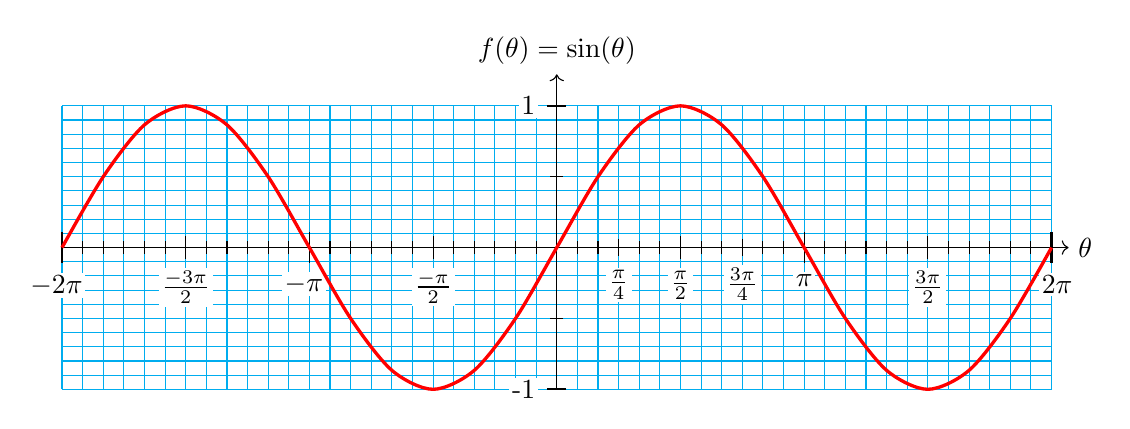
\begin{tikzpicture}

\draw[cyan,xstep=pi/12,ystep=0.18]
(-2*pi,-1.8) grid (2*pi,1.8);

\draw[->] (-6.3,0) -- (6.5,0) node[right] {$\theta$};
\draw[->] (0,-1.8) -- (0,2.2) node[above] {$f(\theta)=\sin(\theta)$};

\foreach \x in {-24,-23,...,24}
\draw[black] ($ pi*\x /12*(1,0) +(0,.08) $) --++(0,-.16);
\foreach \y in {-0.9, 0.9}
\draw[black] (.08,\y ) --++(-.16,0);
\foreach \y in {-1,1}
\draw[black, thick] (.12,1.8*\y ) --++(-.24,0) node[anchor=east, xshift=-3, fill=white, inner sep=1pt] {\y};

\draw[black, thick] (-2*pi,.2) --++(0,-.4) node[anchor=north, xshift=-2,yshift=-3, fill=white, inner sep=1pt] {$-2\pi$};
\draw[black, thick] (2*pi,.2) --++(0,-.4) node[anchor=north, xshift=2,yshift=-3, fill=white, inner sep=1pt] {$2\pi$};

\draw[black] (pi,.2) --++(0,-.4) node[anchor=north, yshift=-3, fill=white, inner sep=1pt] {$\pi$};

\draw[black] (pi,.2) --++(0,-.4) node[anchor=north, yshift=-3, fill=white, inner sep=1pt] {$\pi$};
\draw[black] (-pi,.2) --++(0,-.4) node[anchor=north, xshift=-2,yshift=-3, fill=white, inner sep=1pt] {$-\pi$};
\draw[black] (-pi/2,.15) --++(0,-.3) node[anchor=north, yshift=-3, fill=white, inner sep=1pt] {$\frac{-\pi}{2}$};
\draw[black] (pi/2,.15) --++(0,-.3) node[anchor=north, yshift=-3, fill=white, inner sep=1pt] {$\frac{\pi}{2}$};
\draw[black] (3*pi/2,.15) --++(0,-.3) node[anchor=north, yshift=-3, fill=white, inner sep=1pt] {$\frac{3\pi}{2}$};
\draw[black] (-3*pi/2,.15) --++(0,-.3) node[anchor=north, yshift=-3, fill=white, inner sep=1pt] {$\frac{-3\pi}{2}$};

\draw[black] (pi/4,.11) --++(0,-.22) node[anchor=north, yshift=-4, fill=white, inner sep=1pt] {$\frac{\pi}{4}$};

\draw[black] (3*pi/4,.11) --++(0,-.22) node[anchor=north, yshift=-3, fill=white, inner sep=1pt] {$\frac{3\pi}{4}$};

\draw[domain=-2*pi:2*pi,smooth,variable=\x,red,very thick] plot ({\x},{1.8*sin(deg(\x))});

\end{tikzpicture}
\newline


cosine graph
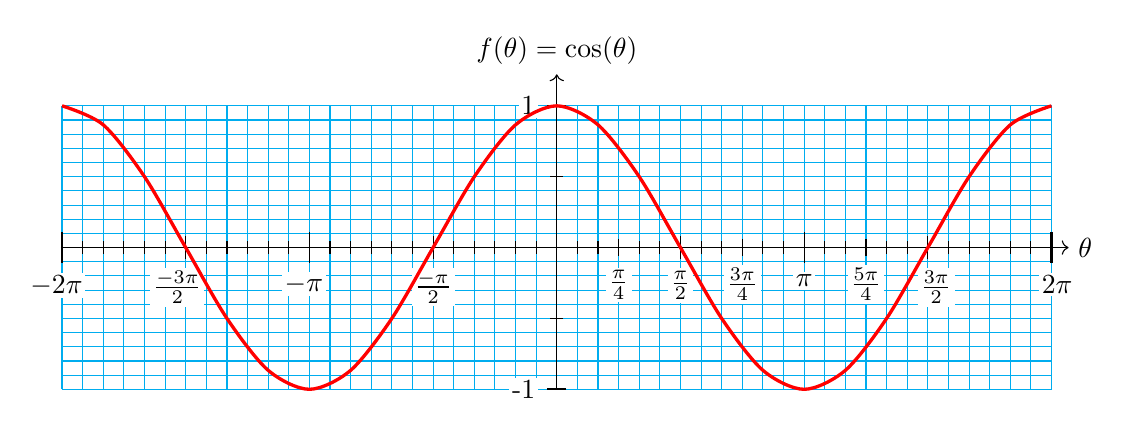
\begin{tikzpicture} 

\draw[cyan,xstep=pi/12,ystep=0.18]
(-2*pi,-1.8) grid (2*pi,1.8);

\draw[->] (-6.3,0) -- (6.5,0) node[right] {$\theta$};
\draw[->] (0,-1.8) -- (0,2.2) node[above] {$f(\theta)=\cos(\theta)$};

\foreach \x in {-24,-23,...,24}
\draw[black] ($ pi*\x /12*(1,0) +(0,.08) $) --++(0,-.16);
\foreach \y in {-0.9, 0.9}
\draw[black] (.08,\y ) --++(-.16,0);
\foreach \y in {-1,1}
\draw[black, thick] (.12,1.8*\y ) --++(-.24,0) node[anchor=east, xshift=-3, fill=white, inner sep=1pt] {\y};

\draw[black, thick] (-2*pi,.2) --++(0,-.4) node[anchor=north, xshift=-2,yshift=-3, fill=white, inner sep=1pt] {$-2\pi$};
\draw[black, thick] (2*pi,.2) --++(0,-.4) node[anchor=north, xshift=2,yshift=-3, fill=white, inner sep=1pt] {$2\pi$};

\draw[black] (pi,.2) --++(0,-.4) node[anchor=north, yshift=-3, fill=white, inner sep=1pt] {$\pi$};

\draw[black] (pi,.2) --++(0,-.4) node[anchor=north, yshift=-3, fill=white, inner sep=1pt] {$\pi$};
\draw[black] (-pi,.2) --++(0,-.4) node[anchor=north, xshift=-2,yshift=-3, fill=white, inner sep=1pt] {$-\pi$};
\draw[black] (-pi/2,.15) --++(0,-.3) node[anchor=north, yshift=-3, fill=white, inner sep=1pt] {$\frac{-\pi}{2}$};
\draw[black] (pi/2,.15) --++(0,-.3) node[anchor=north, yshift=-3, fill=white, inner sep=1pt] {$\frac{\pi}{2}$};
\draw[black] (3*pi/2,.15) --++(0,-.3) node[anchor=north,xshift=3, yshift=-3, fill=white, inner sep=1pt] {$\frac{3\pi}{2}$};
\draw[black] (-3*pi/2,.15) --++(0,-.3) node[anchor=north,xshift=-3, yshift=-3, fill=white, inner sep=1pt] {$\frac{-3\pi}{2}$};

\draw[black] (pi/4,.11) --++(0,-.22) node[anchor=north, yshift=-4, fill=white, inner sep=1pt] {$\frac{\pi}{4}$};

\draw[black] (3*pi/4,.11) --++(0,-.22) node[anchor=north, yshift=-3, fill=white, inner sep=1pt] {$\frac{3\pi}{4}$};

\draw[black] (5*pi/4,.11) --++(0,-.22) node[anchor=north, yshift=-3, fill=white, inner sep=1pt] {$\frac{5\pi}{4}$};

\draw[domain=-2*pi:2*pi,smooth,variable=\x,red,very thick] plot ({\x},{1.8*cos(deg(\x))});

\end{tikzpicture}
\newline


tangent graph
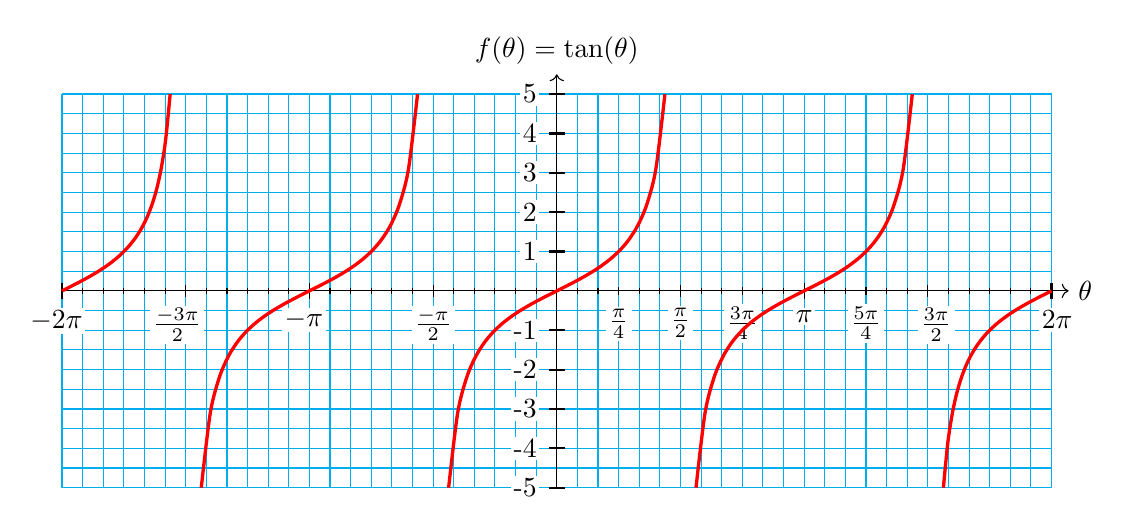
\begin{tikzpicture} [yscale=.5]

\draw[cyan,xstep=pi/12,ystep=0.5]
(-2*pi,-5) grid (2*pi,5);

\draw[->] (-6.3,0) -- (6.5,0) node[right] {$\theta$};
\draw[->] (0,-5) -- (0,5.5) node[above] {$f(\theta)=\tan(\theta)$};

\foreach \x in {-24,-23,...,24}
\draw[black] ($ pi*\x /12*(1,0) +(0,.08) $) --++(0,-.16);
\foreach \y in {-5,-4,...,-1,1,2,...,5}
\draw[black, thick] (.10,\y ) --++(-.2,0) node[anchor=east, xshift=-3, fill=white, inner sep=1pt] {\y};

\draw[black, thick] (-2*pi,.2) --++(0,-.4) node[anchor=north, xshift=-2,yshift=-3, fill=white, inner sep=1pt] {$-2\pi$};
\draw[black, thick] (2*pi,.2) --++(0,-.4) node[anchor=north, xshift=2,yshift=-3, fill=white, inner sep=1pt] {$2\pi$};

\draw[black] (pi,.2) --++(0,-.4) node[anchor=north, yshift=-3, fill=white, inner sep=1pt] {$\pi$};

\draw[black] (pi,.2) --++(0,-.4) node[anchor=north, yshift=-3, fill=white, inner sep=1pt] {$\pi$};
\draw[black] (-pi,.2) --++(0,-.4) node[anchor=north, xshift=-2,yshift=-3, fill=white, inner sep=1pt] {$-\pi$};
\draw[black] (-pi/2,.15) --++(0,-.3) node[anchor=north, yshift=-3, fill=white, inner sep=1pt] {$\frac{-\pi}{2}$};
\draw[black] (pi/2,.15) --++(0,-.3) node[anchor=north, yshift=-3, fill=white, inner sep=1pt] {$\frac{\pi}{2}$};
\draw[black] (3*pi/2,.15) --++(0,-.3) node[anchor=north,xshift=3, yshift=-3, fill=white, inner sep=1pt] {$\frac{3\pi}{2}$};
\draw[black] (-3*pi/2,.15) --++(0,-.3) node[anchor=north,xshift=-3, yshift=-3, fill=white, inner sep=1pt] {$\frac{-3\pi}{2}$};

\draw[black] (pi/4,.11) --++(0,-.22) node[anchor=north, yshift=-4, fill=white, inner sep=1pt] {$\frac{\pi}{4}$};

\draw[black] (3*pi/4,.11) --++(0,-.22) node[anchor=north, yshift=-3, fill=white, inner sep=1pt] {$\frac{3\pi}{4}$};

\draw[black] (5*pi/4,.11) --++(0,-.22) node[anchor=north, yshift=-3, fill=white, inner sep=1pt] {$\frac{5\pi}{4}$};

\foreach \i in {-1, 0, 1}
	\draw[domain={\i*pi-atan(5)*pi/180}:{\i*pi+atan(5)*pi/180}, smooth, variable=\x,red,very thick] plot ({\x},{tan(deg(\x))}) ;

\draw[domain={-2*pi:atan(5)*pi/180-2*pi}, smooth, variable=\x,red,very thick] plot ({\x},{tan(deg(\x))}) ;
\draw[domain={2*pi-atan(5)*pi/180:2*pi}, smooth, variable=\x,red,very thick] plot ({\x},{tan(deg(\x))}) ;

\end{tikzpicture}
\newline


part A: law of sines a circumscribing circle

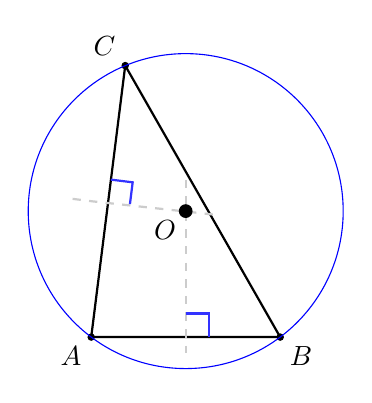
\begin{tikzpicture} [scale=.4]

\coordinate (O) at (0,0);
\coordinate (A) at (-3,-4);
\coordinate (B) at (3,-4);
\coordinate (C) at (-1.92,4.62);

\filldraw (A) circle (.1cm) node[anchor=north east] {$A$};
\filldraw (B) circle (.1cm) node[anchor=north west] {$B$};
\filldraw (C) circle (.1cm) node[anchor=south east] {$C$};

\draw[black,thick] (A)--(B)--(C)--(A);
\draw[gray!40!white, thick, dashed](O)++(0,1) -- (0,-4)--+(0,-.5);
\draw[gray!40!white, thick, dashed](O)++(.862,-.108) -- (-2.96,.31)--++(-.862,.108);
\draw[blue!80!white,thick] (0,-4)++(.75,0)-- ++(0,.75) -- ++(-.75,0);
\draw[blue!80!white,thick] (-2.46,.31) ++(.0864,.6896) -- ++(.6896,-.0864) -- ++(-.0864,-.6896);
\filldraw (O) circle (.2cm) node[anchor=north east] {$O$};

\draw[blue] (O) circle (5);

\end{tikzpicture}
\newline

part B: law of sines a circumscribing circle

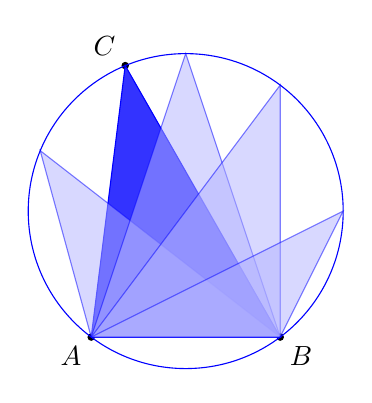
\begin{tikzpicture} [scale=.4]

\coordinate (O) at (0,0);
\coordinate (A) at (-3,-4);
\coordinate (B) at (3,-4);
\coordinate (C) at (-1.92,4.62);
\coordinate (Cp) at (-4.62,1.92);
\coordinate (Cpp) at (0,5);
\coordinate (Cppp) at (3,4);
\coordinate (Cpppp) at (5,0);

\filldraw (O) circle (.1cm) node[anchor=north east] {$O$};
\filldraw (A) circle (.1cm) node[anchor=north east] {$A$};
\filldraw (B) circle (.1cm) node[anchor=north west] {$B$};
\filldraw (C) circle (.1cm) node[anchor=south east] {$C$};

\draw[draw= blue, fill=blue!80!white] (A)--(B)--(C)--(A);
\draw[draw= blue, fill=blue!30!white, opacity=.5] (A)--(B)--(Cp)--(A);
\draw[draw= blue, fill=blue!30!white, opacity=.5] (A)--(B)--(Cpp)--(A);
\draw[draw= blue, fill=blue!30!white, opacity=.5] (A)--(B)--(Cppp)--(A);
\draw[draw= blue, fill=blue!30!white, opacity=.5] (A)--(B)--(Cpppp)--(A);


\draw[blue] (O) circle (5);

\end{tikzpicture}
\newline

Exercise not used?
\begin{tikzpicture}
\coordinate (O) at (0,0);
\coordinate (A) at (0,0);
\coordinate (B) at (0,0);
\coordinate(C) at (0,0);
\coordinate (D) at (0,0);
\filldraw[black] (O) circle (.2pt) node[anchor=south west, xshift=6]{$50\degree$};
\filldraw[black] (A) circle (.2pt) node[anchor=south east]{$x$};
\filldraw[black] (B) circle (.2pt) node[anchor=north east, xshift=-6]{$y$};
\filldraw[black] (C) circle (.2pt) node[anchor=north west]{$z$};
%\draw[black,  thick] (A) -- (B) --( C) -- cycle;
\draw[black] (-2.3,0) --  (2.3,0);
\draw[black] (0.8,1.3) --  (-0.8,-1.3) ;
\end{tikzpicture}
\newline


\end{document}
